\documentclass{emonides-cv}
\usepackage{fontspec}

\setsansfont{Dotum}

\begin{document}
  
\rhead {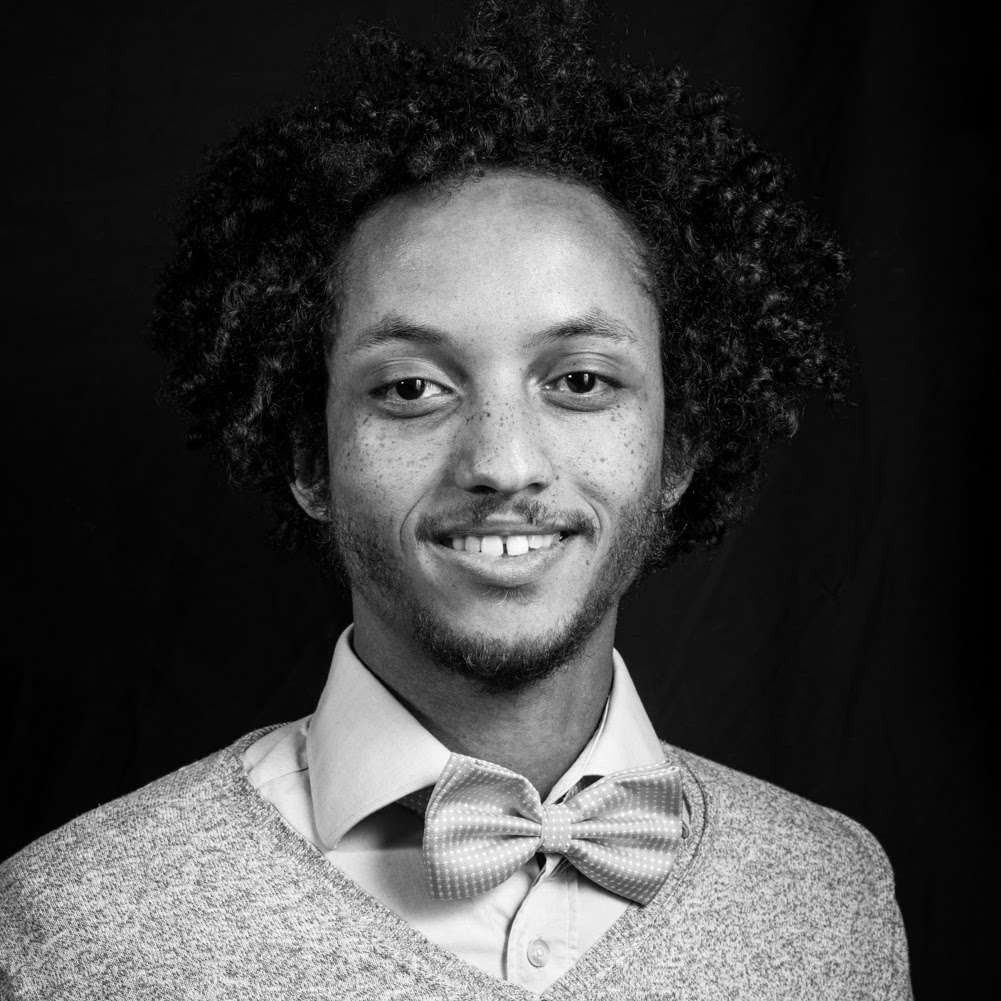
\includegraphics[width=1.5cm]{photoCV.jpg}}
  {Emonides} {Pierre-Emmanuel}
  {Software Engineer/DevOps/MobileDeveloper}
  { 130 Rue de Tolbiac\\
    75013 Paris\\
    France\\
    +33 665 44 88 14\\
    pemonides@gmail.com\\
    }
% \begin{aside}
%   \section{about}
%     130 Rue de Tolbiac
%     75013 Paris
%     France
%     +33 665 44 88 14
%     ~
%   \section{languages}
%     french native
%     english fluent
%     korean notions
%   \section{misc}
%     Driver Licence
% \end{aside}

I'm a full stack software engineer, I have 5+ years experience with backend and mobile development.
I would like to keep working on subjects like DevOps, mobile, on languages like C\# or Python.   
 
\section{Experience}
\begin{entrylist}
  \entry
    {Since  2016}
    {CTO at \href{https://360boost.com/}{360Boost}  {\normalfont Paris}}
    {2years Full Time}
    {\emph{Technical-lead, conception, planning, development and deployment of \textbf{C\# Android/IOS app, NodeJs} Servers.
     Managment of Clusters on \textbf{Gcloud, Kubernetes, Ansible}. Team-lead with 4 employees.(1500 Users, B2B + B2C)
    \\Mobile App
    \\Backend B2B
    \\Api Server}}
  \entry
    {2015}
    {Mobile Consultant, \href{https://www.docapost.com/en/}{Docaposte} {\normalfont Paris}}
    {6 months FullTime}
    {\emph{\textbf{Android/Java Developer}. Sent to a major client of Acensi Docapost, I had to develop on Java/Tomcat servers, as well as mobile applications on \textbf{Java Android}.}}
  \entry
    {2014-2015}
    {Consultant, \href{https://www.acensi.fr/}{Acensi} {\normalfont Paris, La Défense}}
    {1.5 years Fulltime}
    {\emph{\textbf{C\# WPF .Net4.5} development for a Finance Banquing software, \href{https://www.eurocaution.net/}{Eurocaution}.
    I became team-lead for this project (15 developers, 3 teams). 2Weeks Sprints, daily stand-up meetings, sprint retrospective etc...
    \\Then \textbf{C\# Xamarin} Mobile development on a para-medical application. \href{http://www.triacys.com/}{Triacys}.
    I worked on a custom Android Kernel for BeagleBoard, then Android Tablets. I also developped custom userspace-drivers for devices like blood pressure monitor.
    (2 developers). Agile management Method with client review meetings. }}
  \entry
    {2012}
    {C++ developer, \href{https://www.acensi.fr/}{Sogeti High Tech} {\normalfont Rennes, France}}
    {6 months}
    {\emph{\textbf{C++/QT} Developer for an IHM testing solution \href{https://www.eurocaution.net/}{Takt Engine}.
    I had to extend the capabilities of the testing solution. I worked with \textbf{OpenCV} to detect Bad Artefacts during Tests }}
  \entry
    {2010}
    {Lua GameDeveloper, \href{https://www.giantbomb.com/white-birds-productions/3010-5637/}{White Birds} {\normalfont Paris, La Défense}}
    {6 months}
    {\emph{Lua Developer for Point-and-click games, \href{https://www.bigfishgames.com/games/6859/cardboard-castle/}{Cardboard Castle}. \href{https://www.wikiwand.com/fr/White_Birds_Productions}{Last King of Africa}}}
\end{entrylist}

\section{Side Projects}
\begin{entrylist}
  \entry
    {Since  2018}
    {Cryptocurrency exchanges arbitrage bot {\normalfont }}
    {Personal projet}
    {\emph{Part of the development team. Retrieve the orderbook/tick data of different exchanges through websockets for analytics. }}
  \entry
    {Since  2017}
    {\href{https://www.Rentfirst.nl/}{Rentfirst.nl} {\normalfont  (Co-Founder)}}
    {Startup}
    {\emph{Rental housing aggregator for the Amsterdam area}}
  \entry
    {Since  2017}
    {\href{http://www.teamgeny.com/}{Team-Geny} {\normalfont Mobile Developer}}
    {Startup}
    {\emph{}}
  \entry
    {Since  2014}
    {\href{https://play.google.com/store/apps/developer?id=EpicBacon}{EpicBacon} {\normalfont Main-Developer}}
    {Personal projet}
    {\emph{blabla}}
  
\end{entrylist}


\section{Skills}
  \normalsize
  \textbf{C\#, JavaScript, Python} , Java\\
  \textbf { NodeJS, Mobile Development, Xamarin.Forms/Android, WPF/WCF}  \\
  MongoDb, PostgreSQL, MySql\\
  \textbf { Ansible, Kubernetes, Docker}, Nginx, (Arch)Linux/*Bsd \\
  Google Cloud, Azure \\
  Git Workflow, Svn, Jira, Mantis\\
  \LaTeX, Gimp, Photoshop, 3DSMax\\
  \textbf { Certifications: 70-483 Programming in C\# }

\section{Education}
\begin{entrylist}
  \entry
    {2013-2014}
    {Master's degree {\normalfont Computer science }}
    {Epitech European Institute of Information Technology, Paris} {Project-oriented pedagogy : around 40 projects achieved alone or within a team.}
  \entry
    {2012-2013}
    {Student exchange program  {\normalfont  Mobile\&Game development }}
    { {\sffamily 계명대학교} Keimyung University, Daegu South Korea} {}
  \entry
    {2009–2012}
    {Bachelor  {\normalfont Computer Science Programming and software design}}
    {Epitech, Rennes} {}
  \entry
    {2006–2009}
    {French Baccalauréat ES. {\normalfont with honors. }}
    {Lycée Schœlcher, Fort-de-France} { Specialization in mathematics }
\end{entrylist}

\section{Activities}
  Thai boxing, Underwater diving\\
  3D Modeling, Drawing\\
  Skating, MotorBike
  
\end{document}

